\documentclass[a4paper]{oblivoir}
\usepackage{amsmath,amssymb,kotex,kswrapfig,mdframed,paralist}
\usepackage{fapapersize}
\usefapapersize{210mm,297mm,20mm,*,20mm,*}

\usepackage{tabto,pifont}
\TabPositions{0.2\textwidth,0.4\textwidth,0.6\textwidth,0.8\textwidth}
\newcommand\tabb[5]{\par\noindent
\ding{172}\:{\ensuremath{#1}}
\tab\ding{173}\:\:{\ensuremath{#2}}
\tab\ding{174}\:\:{\ensuremath{#3}}
\tab\ding{175}\:\:{\ensuremath{#4}}
\tab\ding{176}\:\:{\ensuremath{#5}}}

\usepackage{graphicx}

%\pagestyle{empty}

%%% Counters
\newcounter{num}

%%% Commands
\newcommand\prob[1]
{\vs\bigskip\bigskip\par\noindent\stepcounter{num} \textbf{문제 \thenum) #1}\par\noindent}

\newcommand\pb[1]{\ensuremath{\fbox{\phantom{#1}}}}

\newcommand\ba{\ensuremath{\:|\:}}

\newcommand\vs[1]{\vspace{40pt}}

\newcommand\an[1]{\bigskip\par\noindent\textbf{문제 #1)}\par\noindent}

%%% Meta Commands
\let\oldsection\section
\renewcommand\section{\clearpage\oldsection}

\let\emph\textsf

\begin{document}
\begin{center}
\LARGE준영, 미니테스트 19
\end{center}
\begin{flushright}
날짜 : 2017년 \(\pb3\)월 \(\pb{10}\)일 \(\pb{월}\)요일
,\qquad
제한시간 : \pb{17년}분
,\qquad
점수 : \pb{20} / \pb{20}
\end{flushright}

%
\prob{}
다항함수 \(f(x)\)가 \[\displaystyle\int(x-1)f(x)\,dx=x^3-3x+C\]를 만족시킬 때, \(f(3)\)의 값은?
(단 \(C\)는 적분상수)
\tabb{10}{12}{14}{16}{18}

%
\prob{}
함수 \(f(x)\)에 대하여
\[f(x)=\int\left\{\frac d{dx}(3x^2+2x)\right\}\,dx\]
이고, \(f(1)=2\)를 만족시킬 때, 방정식 \(f(x)=0\)을 만족시키는 모든 실수 \(x\)의 값의 합은?
\tabb{-\frac53}{-\frac43}{-1}{-\frac23}{-\frac13}

%
\prob{}
함수 \(f(x)\)가 \(f'(x)=9x^2+6x-2\), \(f(0)=3\)을 만족시킬 때, \(f(1)\)의 값은?
\tabb56789

%
\prob{}
\begin{minipage}{0.45\textwidth}
삼차함수 \(f(x)\)의 도함수 \(y=f'(x)\)의 그래프가 그림과 같다.
\(f(0)=2\)일 때, \(f(3)\)의 값은?
\end{minipage}
\begin{minipage}{0.45\textwidth}
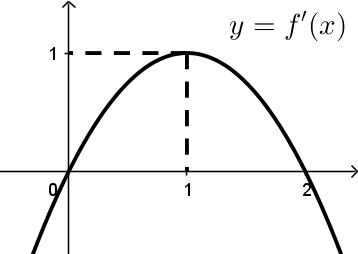
\includegraphics[width=0.5\textwidth]{y=2x-x^2}
\end{minipage}
\tabb{2}{5}{8}{11}{14}

\clearpage
%
\prob{}
함수 \[f(x)=\int\left(1+2\sqrt x\right)^2\,dx+\int\left(1-2\sqrt x\right)^2\,dx\]
에 대하여 \(f(0)=4\)일 때, \(f(1)\)의 값은?
\tabb{8}{9}{10}{11}{12}

%
\prob{}
곡선 \(y=f(x)\)위의 점 \((x,f(x))\)에서의 접선의 기울기가 \(2x-3\)이고 이 곡선이 \((2,4)\)를 지날 때, \(f(1)\)의 값은?
\tabb12345

%
\prob{}
미분가능한 함수 \(f(x)\)가 \(f'(0)=1\)이고 모든 실수 \(x\), \(y\)에 대하여 \(f(x+y)=f(x)+f(y)+xy\)를 만족시킬 때, \(f(4)\)의 값은?
\tabb{10}{11}{12}{13}{14}

%
\prob{}
다항함수 \(f(x)\)가
\[\int_a^xf(t)\,dt=x^2+3x-2\]
를 만족시킬 때, \(f(2)\)의 값은?
(단, \(a\)는 상수이다.)
\tabb34567

%
\prob{}
\(\displaystyle\int_1^2(x^2+4x)\,dx\)의 값은?
\par\medskip\tabb7{\frac{22}3}{\frac{23}3}8{\frac{25}3}

%
\prob{}
\(\displaystyle\int_0^3\frac{x^3}{x+1}\,dx+\int_0^3\frac1{x+1}\,dx\)의 값은?
\par\medskip\tabb{\frac92}{\frac{11}2}{\frac{13}2}{\frac{15}2}{\frac{17}2}

\clearpage
%
\prob{}
함수
\[f(x)=\begin{cases}3x^2+x&(x<1)\\2x+a&(x\ge1)\end{cases}\]
가 모든 실수 \(x\)에서 연속일 때, \(a+\int_{-1}^2f(x)\,dx\)의 값은?
(단, \(a\)는 상수이다.)
\tabb6789{10}

%
\prob{}
\(\displaystyle\int_{-1}^120x^{11}+3x^2+5x+2\,dx\)
의 값은?
\par\medskip\tabb369{12}{15}

%
\prob{}
\(\displaystyle\lim_{x\to2}\frac1{x-2}\int_2^x(t^2-3t+2)\,dt\)의 값은?
\par\medskip\tabb{-1}0123

%
\prob{}
\(\displaystyle\lim_{n\to\infty}\frac1n
\left\{\left(1+\frac1n\right)^2+\left(1+\frac2n\right)^2
+\cdots+\left(1+\frac nn\right)^2\right\}\)
의 값은?
\par\medskip\tabb{\frac73}{\frac52}{\frac83}{\frac{17}6}{3}

\end{document}